\documentclass[ucs, notheorems, handout]{beamer}

\usetheme[numbers,totalnumbers]{Statmod}
\usefonttheme[onlymath]{serif}
\setbeamertemplate{navigation symbols}{}

%\mode<handout> {
%    \usepackage{pgfpages}
%    \setbeameroption{show notes}
%    \pgfpagesuselayout{2 on 1}[a4paper, border shrink=3mm]
%}

\usepackage[utf8x]{inputenc}
\usepackage[T2A]{fontenc}
\usepackage[russian]{babel}
\usepackage{tikz}
\usepackage{ragged2e}
\usepackage{amsthm}
\usepackage{wrapfig}
\usepackage{bm} %bold math
\usepackage{url}
\usepackage{dirtytalk} %for quotes
\usepackage{graphicx}
\usepackage{marginnote}
\usepackage{bm}
\usepackage[makeroom]{cancel}
\usepackage{algorithm2e}
\newcommand{\sign}{\text{sign}}
\DeclareMathOperator*{\argmax}{arg\,max}
\DeclareMathOperator*{\argmin}{arg\,min}
\DeclareMathOperator{\rank}{rank}
\DeclareMathOperator{\diam}{diam}
\DeclareMathOperator{\ob}{Ob}
\DeclareMathOperator{\Hom}{Hom}
\DeclareMathOperator{\var}{Var}
\DeclareMathOperator{\bias}{Bias}
\newcommand{\betah}{\hat{\bm \beta}}
\newcommand{\betaa}{\bm{\beta}}
\newcommand{\epss}{\bm{\varepsilon}}
\newcommand{\E}{\mathrm{E}}
\newcommand{\D}{\mathrm{D}}
\newcommand{\XT}{{\bm{X}}^{\mathrm{T}}}
\newcommand{\X}{\bm{X}}
\renewcommand{\thealgocf}{}
\definecolor{asparagus}{rgb}{0.53, 0.66, 0.42}

\newtheorem{theorem}{Теорема}
\newtheorem{definition}{Определение}
\addto\captionsrussian{\renewcommand{\figurename}{Figure}}
\addto\captionsrussian{\renewcommand{\tablename}{Table}}

\title[Регрессия, регуляризация, отбор признаков]{%
     Регрессия, регуляризация, отбор признаков}

\author[Гоголева, Капаца, Мандрикова]{Елена Гоголева, Дейвид Капаца, Анастасия Мандрикова}

\institute[Санкт-Петербургский Государственный Университет]{%
    \small
    Санкт-Петербургский государственный университет\\
    Прикладная математика и информатика\\
    Вычислительная стохастика и статистические модели\\
    \vspace{1.25cm}
    Семинар по статистическому и машинному обучению}

\date[]{Санкт-Петербург, 2021}

%\subject{Talks}

\begin{document}

\begin{frame}[plain]
    \titlepage

    \note{Начнём.}
\end{frame}


%\section{Характеристика работы}
%\subsection{Общие слова}

%\setbeameroption{show notes}

\begin{frame}
    \frametitle{План доклада}

 \begin{enumerate}
 		 \item Регрессия в общем виде
 			\begin{itemize}
 				\item Какая задача оптимизации решается?
 				\item Выбор функции потерь
 			\end{itemize}
         \item Линейная регрессия
       		\begin{itemize}
 				\item Многомерная постановка, МНК-оценка $\betah$
 				\item Предположения о модели. Остатки
 				\item Критерии
 				\item Особенности вычисления $\betah$
 			\end{itemize}
         \item Регуляризация
       		\begin{itemize}
 				\item Ridge Regression (гребневая регрессия)
 				\item Lasso 
 				\item Некоторые модификации (Elastic Net, RegLAD)
 			\end{itemize}
         \item Отбор признаков
			\begin{itemize}
 				\item Best subset selection
 				\item Forward/Backward selection 
 			\end{itemize}
         \end{enumerate}
    \note{
   С одной стороны, нам досталась известная всем нам тема и сказать в ней что-то новое будет сложновато. 
   \\~\\
   С другой --- нам нужно было сделать доклад так, чтобы из него все могли вынести что-то полезное и новое для себя. 
   \\~\\
   В этот раз будет больше слов про оптимизацию, алгоритмы, пакеты и функции, чем про вероятность и критерии.
   \\~\\
   ДАЛЕЕ ПО СЛАЙДУ
    
}
\end{frame}

\begin{frame}
    \frametitle{Регрессия в ML}


Имеется набор данных (обучающая выборка)
$$
\X \in \mathbb{R}^{n\times p}, \quad \bm y \in \mathbb R^n
$$ 
\vspace{0.5cm}   
$\mathbf x_i \in \mathbb R^p$ --- вектор-строки $\X$, $X_i \in \mathbb R^n$ --- вектор-столбцы $\X$.

\textbf{Задача:} уметь предсказывать $y$ (ответ) по новым $\mathbf x_i$ (объектам), установив некоторую зависимость на обучающей выборке.
\vspace{0.5cm}  

Какие минимальные требования наложить на все $\mathbf x_i$ и $\bm y$?
\begin{block}{Гипотеза непрерывности}
\centering
<<близким>> объектам $\mathbf x_i$ соответствуют  <<близкие>> ответы $y_i$
\end{block}
 
    \note{
    Перейдём к вероятностной постановке задачи регрессии, которая в некотором смысле формализует поставленную задачу
        }
\end{frame}


\begin{frame}
    \frametitle{Регрессия: вероятностная постановка}
    \vspace*{-5mm}
\begin{center}
	\textbf{Генеральная постановка}
\end{center}

$\bm \xi \in \mathbb R^p$ --- случайный вектор, $\eta, \varepsilon \in \mathbb R$ --- случайные величины.

Предполагаем, что $\eta$ и $\bm \xi$ функционально зависимы:
\begin{block}{}
\centering
$\eta = \varphi(\bm \xi) + \varepsilon$
\end{block}
Обычно $\E \varepsilon = 0, \, \D \varepsilon = \sigma^2,\, \bm\xi \perp \varepsilon. $
\begin{center}
\textbf{Переход к выборке}
\end{center}
$\mathbf x_1, \ldots, \mathbf x_n \sim \mathcal L(\bm \xi)$; $y_1, \ldots, y_n \sim \mathcal L(\eta)$ --- выборки, которые наблюдаем.
Модель для всех $i \in 1:n$ 
\begin{block}{}
\centering
$y_i = \varphi(\mathbf x_i) + \varepsilon_i$
\end{block}

\textbf{{\color{blue}{Задача:}}} найти функцию $\varphi$.

    
    \note{
    
    [ПО СЛАЙДУ]
    
    Задача заключается в том, чтобы определить функцию $\varphi$ по выборке.
    }
\end{frame}

\begin{frame}
    \frametitle{Регрессия: этапы обучения модели}
\begin{block}{Модель}
$$
y_i = \varphi(\mathbf x_i) + \varepsilon_i
$$
\end{block}
\textbf{\color{blue}{Задача:}} найти функцию $\varphi$.
\vspace{3mm}
\begin{enumerate}
	\item Выбор модели регрессии (класс рассматриваемых $\varphi(\cdot)$)
	
	{\color{gray} Линейная модель: $\varphi(\mathbf x_i, \betaa) = \sum_{j = 1}^p \beta_i \mathbf x_i[j],\quad i \in 1:n $}
	
	\item Выбор функции потерь (loss function)
	
	{\color{gray} Квадратичная функция потерь: $\sum_{i = 1}^n(y_i - \varphi(\mathbf x_i, \betaa))^2$}
	\item Выбор метода обучения (training)

{\color{gray} МНК: $\betah = \argmin_{\betaa}{\sum_{i = 1}^n(y_i - \varphi(\mathbf x_i, \betaa))^2}$}
	\item Выбор метода проверки (test)

{\color{gray} MSE: $\tfrac{1}{n_{\text{test}}}\sum_{i = 1}^{n_{\text{test}}}(y^{\text{test}}_i - \varphi(\mathbf x_i^{\text{test}}, \betah))^2$}
\end{enumerate}            
    \note{
    Вот как обычно выглядит процесс построения регрессионной модели для выборки. 
    
    Серым цветом для примера выделены соответствующие этапы в классической линейной регрессии.
}
\end{frame}


\begin{frame}
    \frametitle{Задача регрессии как задача оптимизации}
\begin{itemize}
	\item $\X \in \mathbb R^{n \times p}$ --- матрица данных (design matrix)
	\item $\bm y \in \mathbb R^n$ --- вектор ответов
	\item $\betaa \in \mathbb R^d$ --- вектор параметров 
	\item $\bm \varphi(\X, \betaa) := (\varphi(\mathbf x_1, \betaa),\ldots, \varphi(\mathbf x_n, \betaa) )^\mathrm T$ --- функция от выборки и параметров	\item $\mathcal L(\bm \varphi(\X, \betaa), \bm y)$ --- \textit{некоторая} функция потерь\footnote{здесь
	$\mathcal L: \mathbb R^{n} \times \mathbb R^n \rightarrow \mathbb R$
	}
\end{itemize}
Решение задачи регрессии --- вектор коэффициентов $\betah$. 
\begin{block}{}
$$\betah = \argmin_{\betaa}{\mathcal L(\bm \varphi(\X, \betaa), \bm y)}$$
\end{block}

    \note{
    Пока что представляем для примера, что функция потерь квадратичная, стандартная, с другими мы ещё не встретились. Так как успешное решение нашей задачи эквивалентно нахождению минимума указанного функционала, становится важным его вид. В случае линейной регрессии и квадратичной функции потерь у этого минимума есть явный вид, однако при выборе более сложных функций потерь нахождение этого минимума становится непростой задачей.
    }
\end{frame}

\begin{frame}
    \frametitle{Выбор функции потерь}

\textit{Какие варианты есть?}
\begin{itemize}
	\item $\|\bm \varphi(\bm X, \betaa) - \bm y\|^2_2$ --- квадратичная ошибка ($l_2$-норма)
	\item $\|\bm \varphi(\bm X, \betaa) - \bm y\|_1$ --- модуль ошибки ($l_1$-норма)
	\item $\frac{1}{n}\sum_{i \in 1:n}|\varphi(\mathbf x_i, \betaa) - y_i|$ --- MAD (mean absolute deviation)\footnote{аналогично $l_1$, только ф-я нормированa на $n$}
	\item $\sum_{i \in 1:n} H_\delta(\varphi(\mathbf x_i, \betaa), y_i)$ --- функция потерь Хубера
	\item \dots
\end{itemize}
    \vspace{3mm}
\textit{Как выбирать?}
\begin{itemize}
	\item Явный вид решения 
	\item Простота функции $\mathcal L$ для оптимизации
	\item Точность данных/наличие выбросов
	\item Конкретные предположения о распределении остатков $\bm \varepsilon$
	\item Инвариантность решения относительно масштаба/сдвига
\end{itemize}

    \note{

    }
\end{frame}

\begin{frame}
    \frametitle{Линейная регрессия: постановка}
    \textbf{Модель:	} $\bm y = \X \betaa + \epss$
\begin{itemize}
	\item $\bm y \in \mathbb R^n$ --- вектор ответов,  $\epss \in \mathbb R^n$ --- вектор ошибок, $\mathrm E\epss = \bm 0$
	\item $\X \in \mathbb R^{n \times p}$ --- матрица данных (design matrix)
	\begin{itemize}
	\item детерминированная
	\item случайная
	\end{itemize}		
	\item $\betaa \in \mathbb R^p$ --- вектор параметров 
	\end{itemize}

Решение задачи линейной регрессии --- вектор $\betah$. 

\textbf{Классическая задача} (с квадратичной функцией потерь):
\begin{block}{}
$$\betah = \argmin_{\betaa}{\|\bm y - \bm X \betaa\|^2_2}$$
\end{block}

Исходная модель не обязательно линейна: ищем наилучшую аппроксимацию в подпространстве столбцов $\X$.

    \note{
Предположения о модели:

1. Матрица плана неслучайна

2. Матрица $\XT\X$ невырожденна 

3. $\E \varepsilon_i = 0,\, \E \varepsilon_i^2 = \sigma^2 < +\infty,\,  \E \varepsilon_i \varepsilon_j = 0$
    }
\end{frame}

\begin{frame}
    \frametitle{МНК-оценка и её особенности I}
    \begin{block}{Задача}
$$\betah = \argmin_{\betaa}{\|\bm y - \bm X \betaa\|^2_2}$$
\end{block}

\begin{block}{Решение}
$$\betah = (\X^\mathrm{T}\X)^{-1} \X^\mathrm{T} \bm y$$
\end{block}	

\begin{itemize}
	\item[\checkmark] Явный вид решения 
	\item[\checkmark] Простота функции $\mathcal L$ для оптимизации
	\item[!] Точность данных/наличие выбросов
	\item[!] Конкретные предположения о распределении остатков $\bm \varepsilon$
	\item[!] Мультиколлинеарность
	\item[!] $n \geqslant p$, иначе решений бесконечно много
\end{itemize}
    \note{
Здесь тезисно перечислены особенности оценки по МНК, мы пройдёмся по этим пунктам подробнее
    }
\end{frame}

\begin{frame}
     \frametitle{МНК-оценка и её особенности II}
 Для оценок $\betah$ имеет место разложение     \begin{block}{}
$$\mathrm{MSE} = \E(\betaa - \betah)^2 = \underbrace{\mathrm D \betah}_{\text{дисперсия}} + \underbrace{(\mathrm E \betah - \betaa)^2}_{\text{смещение}}$$
\end{block}

Рассмотрим МНК-оценку $\betah = (\X^\mathrm{T}\X)^{-1} \X^\mathrm{T} \bm y$
    
\begin{itemize}
	\item $\E \betah = \betaa$, то есть оценка несмещённая
	\item $\D \betah = \sigma^2 (\XT\X)^{-1}$ (в случае, когда $\varepsilon_i \sim \mathrm N(0, \sigma^2)$)
	\item В классе несмещённых оценок $\betah$ обладает наименьшей дисперсией ($\betah$ --- BLUE)
	\item Если остатки распределены нормально, то $\betah$ --- ОМП
 \end{itemize}


    \note{

    }
\end{frame}


\begin{frame}
    \frametitle{Распределение ошибки $\epss$}
    \textbf{Модель:} $\bm y = \X \betaa + \epss$

\begin{itemize}
	\item Распределение $\epss$ --- нормальное, $\E \epss = \bm 0$:
 \begin{itemize}
 	\item Классическая оценка по МНК --- ОМП и BLUE
	\item Работают стандартные критерии значимости
 \end{itemize}
 		\item Распределение $\epss$ неизвестно или с тяжёлыми хвостами:
 			\begin{itemize}
 				\item Оценка по МНК уже не ОМП и не BLUE
				\item Использование робастных функций потерь, итеративных методов
				\item Проверка качества модели на тестовой выборке
 			\end{itemize}
\end{itemize}

\begin{alertblock}{Вывод}
Анализ остатков необходим!
\end{alertblock}

    \note{

    }
\end{frame}

\begin{frame}
    \frametitle{МНК-оценка: вычислительный взгляд}

\begin{block}{Решение}
$$\betah = (\X^\mathrm{T}\X)^{-1} \X^\mathrm{T} \bm y$$
\end{block}	

\begin{itemize}
\item Необходимо вычислить $\betah$
\item Сингулярное разложение: $\X = \bm V \bm D \bm U^\mathrm T$
\begin{itemize}
\item $\bm V$ и $\bm U$ --- ортогональные, $\bm D$ --- диагональная
\item $\bm V = (V_1, V_2, \ldots, V_n) \in \mathbb R^{n\times n}$, $V_i$ --- с.\,векторы $\X \XT$
\item $\bm U = (U_1, U_2, \ldots, U_n) \in \mathbb R^{p\times n}$, $U_i$ --- с.\,векторы $\XT \X$
\item $\bm D = \mathrm{diag}(\sqrt{\lambda_1}, \ldots,\sqrt{\lambda_n})$, $\lambda_j \geqslant 0$ --- с.\,значения $\XT \X$
\end{itemize}

Отсюда $\betah = \bm U \bm D^{-1} \bm V^\mathrm T\bm y$
\item $\bm D^{-1} = \mathrm{diag} (1/\sqrt{\lambda_1}, \ldots, 1/\sqrt{\lambda_n})$ 
\begin{alertblock}{Что, если $\lambda_j \approx 0$?}
Плохо.
\end{alertblock}
\end{itemize}
    \note{

    }
\end{frame}


\begin{frame}
    \frametitle{Когда $\lambda_i \approx 0$? Мультиколлинеарность}

\begin{itemize}
	\item $\lambda_i$ --- собственные числа $\XT \X$
	\item \textbf{Факт:} Если существует $\bm v \in \mathbb R^p$ такой, что $\X \bm v \approx \bm 0$, то некоторые $\lambda_i \approx 0$
	\item Когда $\X \bm v \approx \bm 0$?\footnote{распишите произведение как линейную комбинацию} {\color{gray}{ Происходит ли такое на практике?}}
	\item Влияние $\lambda_i$ на $\betah$ можно объяснить так:
\end{itemize}

\begin{definition}
$\mu(\bm S) = \|\bm S\|\|\bm S^{-1}\| = {\lambda_{\text{max}}}/{\lambda_{\text{min}}}$ называется \textbf{числом обусловленности} матрицы $\bm S$
\end{definition}

При умножении $\bm S^{-1}\bm v = \bm z$ происходит увеличение погрешности в $\mu(\bm S)$ раз:
$$
\frac{\|\delta \bm z\|}{\|\bm z\|} \leqslant \mu(\bm S) \frac{\|\delta \bm v\|}{\|\bm v\|}
$$
    \note{

    }
\end{frame}

\begin{frame}
    \frametitle{Борьба с мультиколлинеарностью}
\begin{centering}
	\textbf{Мультиколлинеарность ($\XT \X$ плохо обусловлена) влечёт}
\end{centering}

\begin{itemize}
	\item Неустойчивость решения
	\item Высокая дисперсия у $\betah$ $\Rightarrow$ высокая MSE
\end{itemize}
\vspace{0.5cm}
\begin{centering}
	\textbf{Возможные решения проблемы мультиколлинеарности}
\end{centering}


\begin{itemize}
	\item Уменьшение числа признаков (отбор признаков)
	\item Регуляризация
	\item Преобразование признаков
\end{itemize}
    \note{
По слайду

Затем

Итак, вспомнили классическую линейную регрессию и некоторые проблемы, с которыми можно столкнуться на практике. В следующей части подробнее рассмотрим методы борьбы с этими проблемами.
    }
\end{frame}


\begin{frame}
    \frametitle{}

\begin{center}
	\huge {Практика}
	
	\large {Регрессия}
\end{center}

    \note{
Передаю слово Насте и Лене. Они покажут, как можно использовать линейную регрессию для предсказания}
\end{frame}


\begin{frame}
    \frametitle{Регуляризация. Гребневая регрессия}
    \textbf{Модель:} $\bm y = \X \betaa + \epss$
	
	Вернёмся к разложению MSE	
$$\mathrm{MSE} = \E(\betaa - \betah)^2 = \underbrace{\mathrm D \betah}_{\text{дисперсия}} + \underbrace{(\mathrm E \betah - \betaa)^2}_{\text{смещение}}$$
Несмещённая оценка может иметь большую дисперсию и MSE.
	
	Возьмём оценку по МНК и сделаем её смещённой:
	$$\betah_{\text{ridge}} = (\XT \X + \lambda \mathbf I)^{-1}\XT\bm y,\quad \lambda > 0$$
	
	Используем SVD и получим
	$$\betah_{\text{ridge}} = \sum_{i = 1}^n \frac{\lambda_j}{\lambda_j + \lambda} U_j(V_j^\mathrm T\bm y)$$

	Отделили знаменатель от нуля. Устойчивость вычислений повышается.

    \note{
	
    }
\end{frame}

\begin{frame}
    \frametitle{Гребневая регрессия. Дисперсия}
$$\mathrm{MSE} = \E(\betaa - \betah)^2 = \underbrace{\mathrm D \betah}_{\text{дисперсия}} + \underbrace{(\mathrm E \betah - \betaa)^2}_{\text{смещение}}$$

\begin{block}{Оценка по методу гребневой регрессии}
$$\betah_{\text{ridge}} = (\XT \X + \lambda \mathbf I)^{-1}\XT\bm y,\quad \lambda > 0$$
\end{block}	

\textit{Смещение} контролируется параметром $\lambda$.
	
	\textit{Что с дисперсией?}
	
	\begin{itemize}
		\item $\betah_{\text{ridge}} = \sum_{i = 1}^n \frac{\sqrt{\lambda_j}}{\lambda_j + \lambda} U_j(V_j^\mathrm T\bm y)$
		\item $\lambda_j$ убывают
		\item $\frac{\sqrt{\lambda_j}}{\lambda_j + \lambda}$ штрафуют компоненты с наименьшей дисперсией
		\item  $\D \betah$ уменьшается $\, \Rightarrow \,$  MSE $\downarrow$
	\end{itemize}
	

    \note{
	
    }
\end{frame}

\begin{frame}
    \frametitle{Гребневая регрессия как задача оптимизации}
Есть две эквивалентные формулировки:
\begin{block}{Ridge Regression}
$$\betah_{\text{ridge}}(\lambda_1) = \argmin_{\betaa}{\|\bm y - \X\betaa\|^2_2 +\lambda_1 \|\betaa\|^2_2}
$$
$$
\betah_{\text{ridge}}(\lambda_2) = \argmin_{\betaa}{\|\bm y - \X\betaa\|^2_2 \text{, s.t. } \|\betaa\|^2_2 \leqslant \lambda_2}
$$
\end{block}	

\textbf{Явное решение} --- уже видели.

\textbf{Демо:} \url{https://www.desmos.com/calculator/3fp4awzeyp}

    \note{
	
    }
\end{frame}

\begin{frame}
  \frametitle{Гребневая регрессия. Выбор параметра}
  
\begin{columns}
    \begin{column}{0.47\textwidth}
$$\betah_{\text{ridge}} = (\XT \X + \lambda \mathbf I)^{-1}\XT\bm y$$

Выбор параметра осуществляется с помощью кросс-валидации.
\\~\\
\textit{На рисунке:}

\color{red}{MSE}

\color{asparagus}{Дисперсия оценки $\betah_\text{ridge}$}

\color{black}{Смещение оценки $\betah_\text{ridge}$}



    \end{column}
    \begin{column}{0.5\textwidth}
            \begin{figure}[]
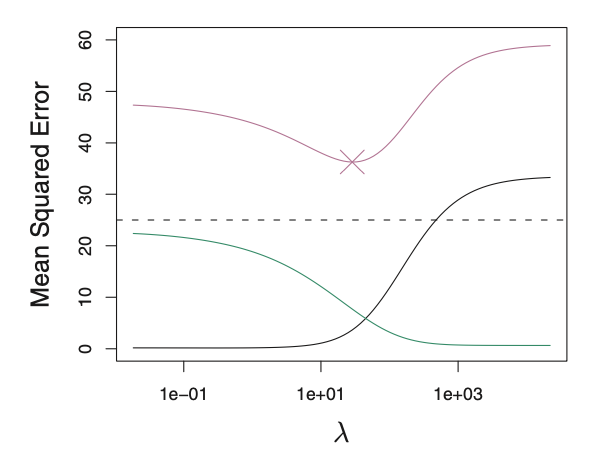
\includegraphics[width=1.1\textwidth]{ridge2.png}
\end{figure}
\end{column}
\end{columns}
    \note{
	
    }
\end{frame}

\begin{frame}
    \frametitle{Регуляризация. Lasso}
Есть две эквивалентные формулировки (явного вида нет):
\begin{block}{Lasso}
$$\betah_{\text{Lasso}}(\lambda_1) = \argmin_{\betaa}{\|\bm y - \X\betaa\|^2_2 +\lambda_1 \|\betaa\|^2_1}
$$
$$
\betah_{\text{Lasso}}(\lambda_2) = \argmin_{\betaa}{\|\bm y - \X\betaa\|^2_2 \text{, s.t. } \|\betaa\|^2_1 \leqslant \lambda_2}
$$
\end{block}	
\textbf{
Особенности:
}
\begin{itemize}
	\item Уменьшение MSE
	\item Интерпретируемость результатов
	\item Быстрое вычисление $\betah_\text{Lasso}(\lambda)$
	\item Случай $p>n$
	\item Выбор параметра: кросс-валидация
\end{itemize}
    \note{
    }
\end{frame}

\begin{frame}
    \frametitle{Регуляризация. Другие методы и подходы}

\begin{itemize}
	\item Elastic net (совмещение Lasso и Ridge)
	\item Использование других норм ($l_q$)
	\item Робастные функции потерь
\end{itemize}
    \note{
	
    }
\end{frame}


\begin{frame}
    \frametitle{Отбор признаков. Общий подход к выбору модели}

Предположим, что есть некоторое семейство построенных моделей $\{\mathcal M_i\}_{i \in I}$.

Хотим выбрать лучшую модель $\mathcal M^*$ для предсказания.

\begin{center}
	\textbf{Классические методы выбора модели}
\end{center} 

\begin{itemize}
	\item Кросс-валидация
	\begin{itemize}
		\item leave-one-out CV
		\item $k$-fold CV
	\end{itemize}
	\item Информационные критерии и $R^2$
	\begin{itemize}
	\item AIC
	\item BIC
	\item $R^2$
	\item $\text{adj.}R^2$ 
	\end{itemize}

\end{itemize}

    \note{
	Говорили, что ещё один способ уменьшить среднеквадратическую ошибку --- выбор переменных.
	\\~\\
	Про кросс валидацию: что меняется при увеличении размера фолда
	
	Про информационные критерии:
	\begin{itemize}
		\item предполагают возможность нахождения $\hat \sigma^2$
		\item плохо работают при увеличении $p$, например $R^2$ увелич. до 1.
		\item Пример того, как это выглядит (график на доске)

	\end{itemize}
	
	When we perform LOOCV, we are in effect averaging the outputs of n fitted models, each of which is trained on an almost identical set of observations; therefore, these outputs are highly (positively) correlated with each other. When we perform k-fold CV with k < n, we are averaging the outputs of k fitted models that are somewhat less correlated with each other. The test error estimate resulting from LOOCV tends to have higher variance than does the test error estimate resulting from k-fold CV.
	
    }
\end{frame}

\begin{frame}
    \frametitle{Отбор признаков. BSS, Forward, Backward}
\begin{itemize}
	\item Best Subset Selection {\color{gray} p = 20: $2^p = 1,048,576$ моделей}
	\item Жадные (greedy) методы
		\begin{itemize}
		\item Forward Stepwise Selection {\color{gray} p = 20: $p(p+1)/2  + 1 = 211$}
		\item Backward Stepwise Selection
		\end{itemize}
	\end{itemize}
    \note{
    пример, когда forward не сработает
    }
\end{frame}

\begin{frame}
    \frametitle{}

\begin{center}
	\huge {Практика}
	
	\large {Регуляризация и отбор параметров}
\end{center}

    \note{
    
    }
\end{frame}


\begin{frame}
    \frametitle{Источники}
\begin{itemize}
	\item ESL (Elements of Statistical Learning) --- Hastie, Tibshirani, Friedman
	\item ISLR (An Introduction to Statistical Learning) --- James, Witten, Hastie, Tibshirani
	\item Лекции Н.Э. и А.И.
	\item Лекции Воронцова по ML
	\item Лекции Larry Wasserman --- Statistical Learning
	\item All of Statistics --- Larry Wasserman
		\end{itemize}
    \note{
    
    }
\end{frame}



%\begin{frame}
%
%Пусть $\betah$ --- оценка вектора коэффициентов. 
%
%\begin{block}{Проблема дисперсии--смещения}
%$$\mathrm{MSE} = \E(\betaa - \betah)^2 = \underbrace{\mathrm D \betah}_{\text{дисперсия}} + \underbrace{(\mathrm E \betah - \betaa)^2}_{\text{смещение}}$$
%\end{block}
%
%
%    \note{
%
%    }
%\end{frame}
%
%
%\begin{frame}
%     \frametitle{Sparsity}
%    \begin{block} {Definition}
%        $\bm \beta = (\beta_1, \ldots, \beta_p)^\mathrm{T}$ --- coefficient vector. Vector of \textbf{significant} regressors is a vector $\bm{\tilde \beta} := \left( \beta_i : \beta_i \neq 0 \right)^\mathrm{T}$. Number of significant regressors: $k := |\bm{\tilde \beta}|$.
%    \end{block}
%    
%    \textbf{Sparse model}: $k \ll p$
%    \begin{itemize}
%        \item \say{Bet on sparsity} principle;
%        \item Examples of sparse problems (Hastie et. al., 2015):
%            \begin{itemize}
%                \item Cancer classification: $n = 349$, $p \approx 70\,000$; $k = 254$ 
%                \item Compressed Sensing: $n = 96\,000$, $p = 1\,000\,000$; $k = 25\,000$.
%            \end{itemize}
%    \end{itemize}
%    
%    \note{
%    As we just said, the first problem is the dimensionality of the parameter space.
%    We will call significant only those coefficients that are not equal to zero. Also, let $k$ be the number of such non zero coefficients. \\~\\
%    We make an assumption that the data is sparse, which means that the sparsity of the model is significantly less than the dimension of the parameter space.
%    This conjecture is based upon the well known "bet on sparsity"  principle meaning that if we assume that all of the regressors are significant, the variance of the calculated estimator would render it useless for practical purposes. \\~\\
%    Listed here are some common examples of sparse problems. They emerge in a variety of fields, including statistics, medicine, signal and image processing.
%}
%\end{frame}
%
%\begin{frame}
%     \frametitle{Two problems: LASSO \& RLAD}
%    %{\color{gray} \textit{Вычислительная сложность построения моделей с разным числом регрессоров}}\\~\\
%    %В предположении разреженности модели ($\tilde p \ll p$), рассмотрим
%    \begin{block} {LASSO (R. Tibshirani, 1996)}
%        \begin{equation*}
%            {\bm{\hat{\beta}}} = \argmin_{\bm \beta}{\underbrace{\|\bm y - \bm{X}\bm\beta\|_2^2}_{\textrm{loss}} + \underbrace{\lambda \|\bm \beta\|_1}_{\textrm{penalty}}} \textrm{, } \lambda \in \mathbb{R}_+ 
%        \end{equation*}
%    \end{block} 
%    
%    \begin{block} {RLAD (Wang, Gordon, Zhu, 2006)}
%\begin{equation*}
%    {\bm{\hat{\beta}}} = \argmin_{\bm \beta}{\underbrace{\|\bm y - \bm{X}\bm\beta\|_1}_{\textrm{loss}} + \underbrace{\lambda \|\bm \beta\|_1}_{\textrm{penalty}}} \textrm{, } \lambda \in \mathbb{R}_+ 
%\end{equation*}
%\end{block}
%    
%    \begin{itemize}
%        \item Regularization parameter $\lambda$ influences the sparsity of the resulting model
%        \begin{itemize}
%            \item $\lambda \rightarrow \infty$ corresponds to $\bm{\beta} = \bm{0}$
%            \item $\lambda = 0$ corresponds to the LSE/LAD
%        \end{itemize}
%        \item Solution path
%        %Существуют пакеты программ, позволяющие построить весь solution path за время, сопоставимое с построением
%    \end{itemize}
%    
%       \note{
%       So, there is a question of whether a certain regressor can be considered insignificant and its coefficient should be set to zero.
%       
%       Consider two problems of sparse regularization: LASSO is based upon the minimization of a target function with $l_2$ norm as a loss function. RLAD is similar, but with the $l_1$ loss function.
%       
%       In both problems each distinct $\lambda$ gives rise to a new optimization problem. For example, when $\lambda \rightarrow \infty$ all coefficients would be equal to zero, whereas when $\lambda = 0$ we get the classical Least Squares and Least Absolute Deviations problems.
%
%The family of models, parametrized by $\lambda$, is called a solution path.
%
%}
%\end{frame}
%
%\begin{frame}
%    \frametitle{Features of RLAD}
%    
%        \begin{block} {RLAD (Wang, Gordon, Zhu, 2006)}
%\begin{equation*}
%    {\bm{\hat{\beta}}} = \argmin_{\bm \beta}{\underbrace{\|\bm y - \bm{X}\bm\beta\|_1}_{\textrm{loss}} + \underbrace{\lambda \|\bm \beta\|_1}_{\textrm{penalty}}} \textrm{, } \lambda \in \mathbb{R}_+ 
%\end{equation*}
%\end{block} 
%    
%   \begin{itemize}
%        \item Low $l_2$-error: $\|\betaa - \betah \|_2^2= \mathcal{O}\left(\sqrt{\frac{k \log p}{n}}\right),$ \newline condition: symmetrical distribution of $\epss$ (L.\,Wang, 2013)
%       \item Solution path algorithm (Wang, Gordon, Zhu, 2006)
%	   \item Problem: choice of $\lambda$ \\L.~Wang (2013) $\hat \lambda = \sqrt{2 n \log p}$
%   \end{itemize}
%     \note{
%We will now quickly list some known facts about RLAD.
%
%First, use of RLAD leads to a low $l_2$ error on the condition that the error is distributed symmetrically. Thus, the resultant estimator is close to the oracle estimator.
%
%The second fact is that there exists a relatively fast algorithm,  which can find the whole solution path in one run.
%
%The main problem of RLAD is finding such parameter $\lambda$ that would lead to the smallest estimation error but at the same time would keep the model sparse. In 2013, Lie Wang proposed to use the value shown on the slide. This choice does not depend on the distribution of error and conditions on the design matrix.
%}
%   
%\end{frame}
%
%\begin{frame}
%\frametitle{Problem statement}
%\begin{enumerate}
%    \item Comparative analysis: LASSO \& RLAD
%    \item Statistical analysis of cross validation for parameter selection
%    \item Modification of the selection method based upon L.\,Wang's paper (2013)
%    \item Application of RLAD and the parameter selection method to image processing
%\end{enumerate}
%\note{ We will now turn to the problem statement.
%
%$\bullet$ First, we had to motivate the usage of the RLAD method by showing its performance under severe noise conditions compared with the LASSO method.
%
%$\bullet$ After that we can turn to the parameter selection problem and numerically analyze the cross–validation and L.Wang's proposed selection method. 
%
%$\bullet$ The main goal was to propose a new modification, which would have a higher computational speed and low prediction error.
%
%$\bullet$ And, in order to provide some applications of the method, an image restoration problem was explored
%}
%\end{frame}

%\begin{frame}
%\frametitle{Моделирование. Общая схема}
%\begin{enumerate}
%\item Создание регрессионной модели с малым числом параметров $\tilde{p}$ (реальная модель)
%\item Добавление в реальную модель множества параметров, не~оказывающих влияние на вектор наблюдений $\bm y$
%\item Искажение вектора результатов $\bm y$ шумом $\bm \varepsilon$
%\item Использование реальной модели для установления ошибки метода  
%\end{enumerate}
%\note{ 
%На данном слайде приводится схема моделирования, которая использовалась при построении. 
%
%\begin{itemize}
%    \item Моделирование повторяется $N = 50$ раз, результаты усредняются
%    \item Для нахождения траекторий решений задачи LASSO используется пакет \texttt{glmnet} для \textsf{R}
%    \item Для нахождения траекторий для LAD-LASSO используется собственная реализация алгоритма Wang, Gordon, Zhu на \textsf{R}
%\end{itemize}
%
%}
%\end{frame}

%\begin{frame}{Моделирование. Небольшой пример}
%Пусть $\tilde{p} = 2$, $p = 4$, $n = 2$, $x_{ij} \sim \textrm{N}(0,1)$, $\delta_i \sim \textrm{Cauchy}(0,1)$ --- все независимы. \\
%Пусть \, $\begin{cases}
%y_1 = 1 \cdot x_{11} + 1 \cdot x_{12} \\ y_2 = 1 \cdot x_{21} + 1 \cdot x_{22}
%\end{cases}$ --- реальная модель.
%
%Добавляем два параметра к модели так, что $y_i = 1\cdot x_{i1}+ 1\cdot x_{i2} + 0 \cdot x_{i3} + 0 \cdot x_{i4} $. \newline Рассмотрим искажённую модель ($\tilde{y}_i = y_i + \delta_i$):
%
%$\begin{cases}
%\tilde{y}_1 = \beta_{1} x_{11} + \beta_{2} x_{12} + \beta_{3} x_{13} + \beta_{4} x_{14} \\
% \tilde{y}_2 = \beta_{1} x_{21} + \beta_{2} a_{22} + \beta_{3} a_{23} + \beta_{4} a_{24}
%\end{cases}$
%
%Хотим, чтобы оценка вектора коэффициентов $\bm \beta$ методами регуляризации была наиболее близка к реальной модели ($\hat{\beta}_1 = 1$, $\hat{\beta}_2 = 1$, $\hat{\beta}_3 = 0$, $\hat{\beta}_4 = 0$).
%\note{ 
%На данном слайде приводится пример моделирования в условиях шума, распределённого по Коши. У данного распределения не существует моментов, что не позволяет применять большинство методов регрессии, основанных на минимизации $l_2$ нормы, в частности МНК и LASSO. Тем не менее, распределение Коши часто встречается в финансовых приложениях, а также в области обработки сигналов
%}
%\end{frame}

%\begin{frame}
%\frametitle{Model quality criteria}
%\begin{enumerate}
%\item Prediction error: $\mathcal{L}_\text{pred}(\betah, \betaa) = \frac{1}{n}\| \X \betah - \X \betaa \|^2_2, $
%\item $l_2$-error: $ \mathcal{L}_2(\betah, \betaa) = \| \betah -  \betaa \|^2_2. $
%\item Type I error ($\hat  \alpha_1 = \frac{k-\hat p_\text{true}}{k}$)
%\item Type II error  ($\hat \alpha_2 = \frac{\hat p_\text{false}}{p - k}$)
%\end{enumerate}
%
%$\hat p_\text{true}$ --- correctly determined to be non-zero,
%$\hat p_\text{false}$ --- incorrectly determined to be non-zero, $k$ - sparsity of the model, $p$ - number of parameters
%\note{
%
%We will now share with you some of the results of our research. \\~\\
%(FAST)
%Here are the main quality criteria we used. \\~\\
%
%Prediction error is the most common measure of estimator quality.
%At the same time, in signal processing, where \textbf{approximating} the vector is primal, $l_2$ error is more useful.
%
%Surely, we would also need ways of estimating the sparsity of the model. To that end, we use type I and type II errors.}
%\end{frame}
%
%\begin{frame}{Results: LASSO vs. RLAD}
%
%    $N_\text{mod} = 50$, $p = 100$, $k= 5$, $n = 100$, $\X$ - Toeplitz matrix, $\beta = (1, 1, 1, 1, 1, 0, \ldots, 0)^\mathrm{T}$, $\epss_i \sim \textrm{Cauchy}(0,1)$ --- all independent.
%
%
%\begin{table}[]
%\begin{tabular}{|l|l|l|l|l|l|l|l|l|}
% \hline
%& $\mathcal{L}_\text{pred}^\text{lad}$ & $\mathcal{L}_\text{pred}^\text{lasso}$ & $\mathcal{L}_2^\text{lad}$ & $\mathcal{L}_2^\text{lasso}$ & $\alpha_1^\text{lad} $ & $\alpha_2^\text{lad} $ & $\alpha_1^\text{lasso} $ & $\alpha_2^\text{lasso} $ \\ 
% \hline
%mean & 0.52 & 20.3 & 0.58 & 17.9 & 0.004 & 0.12 & 0.64 & 0.04 \\ 
%\hline
%  sd & 0.34 & 39.6 & 0.38 & 38.9 & 0.028 & 0.06 & 0.36 & 0.04 \\ 
% \hline
%\end{tabular}
%\caption{Averages of errors across various criteria, LASSO vs. RLAD} 
%\end{table}
%
%\begin{itemize}
%    \item Significant reduction in error
%    \item Correct identification of almost all non-zero coefficients
%\end{itemize}
%
%\note{
%In order to compare LASSO and RLAD, we have performed numerical analysis. Major conditions are outlined here, as you can see the noise term comes from the Cauchy distribution, which does not have any moments. 
%
%I also have to say that in our paper we have detailed discussions of numerical experiments for a variety of conditions.
%
%We have concluded that under such challegning conditions the resulting RLAD estimator can boast a relatively low prediction error and low type I and type II errors.
%
%Now, after some promising results on the method, we turn to the parameter selection problem.
%}
%
%\end{frame}
%
%
%\begin{frame}{Results: cross-validation}
%  
%$N_\text{mod} = 50$, $p = 100$, $k= 5$, $n = 100$, $\X$ - Toeplitz matrix, $\beta = (1, 1, 1, 1, 1, 0, \ldots, 0)^\mathrm{T}$, $\epss_i \sim \textrm{Cauchy}(0,1)$ --- all independent.
%
%    \begin{figure}
%        \centering
%            \includegraphics[width=\linewidth]{cauchy_cv.pdf}
%    \end{figure}
%    
%     \note{
%     To such purpose we have performed a 5 fold cross validation and did 50 modellings for various distributions of the error term. The scheme is almost identical to the already mentioned setup.
% \\~\\
%
%You can see the plot of a typical modelling, when the cross validation error curve approximates the error curve quite well and its minimum provides a reasonable estimate of the best parameter
%
%We will skip numerical results for cross validation and go straight to its modification that we have proposed.}
%\end{frame}
%
%\begin{frame}{Modification of the cross-validation method}
%\begin{itemize}
%
%    \item L.~Wang (2013): $$\hat \lambda(C) = \sqrt{C n \log p},$$
%    \item A limited number of models: $\lambda_i = \lambda(C_i),\, i = 1, \ldots, m$
%    \item Using cross-validation on a smaller set of $\{\lambda_i\}$:   no need to calculate the solution path
%\end{itemize}
%
%\note{
%It was determined by Lie Wang in 2012 that in order to get a good quality estimator we could use the family of parameters shown on the slide.
%So the idea of the modification is to do cross–validation on a much smaller set of parameters based upon this theoretical fact. This in fact provides a much faster procedure and in the end we get a good estimator with a low prediction error.
%}
%
%\end{frame}
%
%\begin{frame}{Results: Modification of the CV metod}
%$N_\text{mod} = 50$, $p = 100$, $k= 5$, $n = 100$, $\X$ - Toeplitz matrix, $\beta = (1, 1, 1, 1, 1, 0, \ldots, 0)^\mathrm{T}$, $\epss_i \sim \textrm{Cauchy}(0,1)$ --- all independent.
%
%\begin{table}
%\centering
%\begin{tabular}{|r|rrr|}
%  \hline
% & $\mathcal M ^\text{best}$ & $\mathcal M ^\text{cvmod}$ & $\mathcal M ^\text{wang}$ \\ 
%  \hline
%mean & 0.517 & 0.645 & 1.933 \\ 
%  sd & 0.417 & 0.497 & 1.635 \\ 
%  min & 0.036 & 0.045 & 0.270 \\ 
%  max & 2.018 & 2.671 & 9.784 \\ 
%   \hline
%\end{tabular}
%\caption{Prediction error for two methods of parameter selection,  case $\epss \sim \mathrm{Cauchy}(0, 1)$; $50$ modellings.} 
%\label{tab:icv_cauchy}
%\end{table}
%
%
%\begin{itemize}
%    \item Greatly reduced prediction error L.\,Wang
%    \item Low computational complexity compared to classical CV
%\end{itemize}
%
%\note{
%
%$\bullet$ Actually, you can see here in the modelling results (second column) that the prediction error is quite close to the least possible error in the first column and significantly better than the error delivered by the method that was proposed earlier
%
%$\bullet$ These results are comparable with cross validation method but I want to underline that computational time for our method decreases dramatically, up to the factor of 10.
%}
%
%\end{frame}
%
%
%\begin{frame}{Results: Applicaton of the RLAD Method I}
%
%\begin{itemize}
%    \item Image restoration problem, noisy picture
%    \item Principal Components Method (PCA)
%\end{itemize}
%
%\begin{figure}[H]
%        \centering
%        \begin{minipage}{\textwidth}
%            \centering
%            \includegraphics[width=0.7\linewidth, page = 3]{bush_train.pdf}
%        \end{minipage}%
%        \caption{A few $64 \times 64$ images from the training set. }  
%		\label{fig:bush_train}
%\end{figure} 
%
%\note{
%
%Of course I wanted to show you some of the applications of this method. So we will now provide a short description of how RLAD can be applied to image reconstruction.
%
%$\bullet$ What is the problem? We have a collection of images of one person \say{in the wild}. The goal is to restore a very noisy picture of the same person using principal components of the training images.
%
%$\bullet$  You can see here some images from the training set. I would like to point out that these images are quite different from each other: I mean lighting conditions, emotions, and even the orientation of the face, which significantly increase the complexity of the problem.
%
%$\bullet$ For each image from the training set of 200 images we have calculated their first 20 principal components. Thus, we make an assumption that the restored image is a linear combination of these components.
%}
%
%\end{frame}
%
%\begin{frame}{Results: Applicaton of the RLAD Method II}
%
%
%\begin{figure}[H]
%        \centering
%        \begin{minipage}{\textwidth}
%            \centering
%            \includegraphics[width=0.2\textwidth]{bush_test.pdf} 
%            \includegraphics[width=0.2\textwidth]{bush_ideal.pdf} 
%   			 \includegraphics[width=0.2\textwidth]{bush_noise_bad.pdf}
%   			 \includegraphics[width=0.2\textwidth]{restored_cauchy_bad.pdf}
%        \end{minipage}%
%        \caption{Original image $\bm B$, its <<best>> approximation using the components, the \say{noisy} variant $\bm B_\text{noisy}$, and the restored image $\hat{\bm B}$.}  
%		\label{fig:bush_final}
%\end{figure} 
%
%\begin{figure}[H]
%        \centering
%        \begin{minipage}{\textwidth}
%            \centering
%
%   			 \includegraphics[width=0.15\textwidth]{bush_noise_cauchy.pdf}
%   			 \includegraphics[width=0.15\textwidth]{restored_cauchy_lo.pdf} \quad
%   			 \includegraphics[width=0.15\textwidth]{bush_text_lo.pdf}
%   			 \includegraphics[width=0.15\textwidth]{bush_restored_text_lo.pdf}
%        \end{minipage}%
%        \caption{$\bm B_\text{noisy}^\text{Cauchy}$ together with its restored version and $\bm B_\text{noisy}^\text{text}$ with its restored version.}  
%		\label{fig:bush_more}
%\end{figure} 
%
%\note{
%
%And here are the results:
%
%$\bullet$ In the first row, from left to right, you can see the original image, it's best fit using the components on the clean version, the noisy image, and its reconstruction. Considering the level of destruction, this can be considered a satisfactory result.
%
%$\bullet$ Below are two more cases of reconstruction, when the noise is not as overwhelming, and the non–random case. 
%
%We can see, that robustness of the method helps restore such images with acceptable quality. 
%}
%
%\end{frame}
%
%
%\begin{frame}{Main results and plans}
%\textbf{Main results}
%\begin{itemize}
%    \item Completed the comparative analysis of LASSO and RLAD
%    \item Applied the cross-validation method for parameter selection
%    \item Proposed a modification of the CV method based on theoretical results
%    \item Applied RLAD and the modified method to the image restoration problem
%\end{itemize}
%
%\textbf{Further plans}
%\begin{itemize}
%	\item Comparison with other methods of sparse regression
%    \item Parameter selection: other methods
%\end{itemize}
%
%\note{
%
%Sadly, we are now coming to the conclusion of this talk.
%You can now see the list of main results and further plans of research.
%
%Thank you very much for your time.
%Please don't hesitate to ask questions if you have any.
%}
%
%\end{frame}
%
%% \begin{frame}{Результаты: LASSO vs. LAD-LASSO IV}
%%     \textbf{Случай с прямоугольной матрицей:}
%    
%%     $p = 100$, $\tilde{p} = 3$, $n = 50$, $x_{ij} \sim \textrm{N}(0,1)$, $\varepsilon_i \sim \textrm{N}(0,0.1)$, $\delta_i \sim 10 \cdot \textrm{B}(1,\,0.05)$ --- все независимы.
%    
%%     \begin{table}[]
%% \begin{tabular}{l|c|c|c|c|c|c|}
%% \cline{2-7}
%%                                 & \multicolumn{2}{c|}{\begin{tabular}[c]{@{}c@{}}Ошибка\\ предсказания\end{tabular}} & \multicolumn{2}{c|}{\begin{tabular}[c]{@{}c@{}}Число\\ угаданных\end{tabular}} & \multicolumn{2}{c|}{\begin{tabular}[c]{@{}c@{}}Число\\ ненулевых\end{tabular}} \\ \cline{2-7} 
%%                                 & mean                                     & sd                                      & mean                                   & sd                                    & mean                                   & sd                                    \\ \hline
%% \multicolumn{1}{|l|}{LASSO}     & 32.37                                    & 16.71                                   & 2.74                                   & 0.53                                  & 46.48                                  & 10.60                                 \\ \hline
%% \multicolumn{1}{|l|}{LAD-LASSO} & 2.52                                     & 0.79                                    & 3                                      & 0                                     & 15.24                                  & 6.53                                  \\ \hline
%% \end{tabular}
%% \end{table}
%% \end{frame}
%
\end{document}
